\documentclass[a0,final]{a0poster}
%%%Load packages
\usepackage{multicol} 			%3-column layout
\usepackage[left=2cm,right=2cm,bottom=0cm,top=0cm]{geometry}			%Reset margins
\usepackage{mathpazo}			%Load palatino font & pazo math
\usepackage{color}				%Needed for colour boxes & coloured text
\usepackage{graphicx}
\usepackage[font = footnotesize, skip=5pt]{caption}
\usepackage{ragged2e}

%%%Define colours and lengths
\definecolor{headingcol}{rgb}{1,1,1}			%Colour of main title
\definecolor{boxcol}{rgb}{0.7,0.2,0.2}		%Edge-colour of box and top banner
\fboxsep=1cm							%Padding between box and text
\setlength{\columnsep}{2cm}				%Set spacing between columns

%%%Format title
\makeatletter							%Needed to include code in main file
\renewcommand\@maketitle{%
\null									%Sets position marker
{
\color{headingcol}\sffamily\VERYHuge		%Set title font and colour
\@title \par}%
\vskip 0.6em%
{
\color{white}\sffamily\Large				%Set author font and colour
\lineskip .5em%
\begin{tabular}[t]{l}%
\@author
\end{tabular}\par}%
\vskip 1cm
\par
}
\makeatother

\title{Drought Variability and the Robustness of Agrarian Social Networks}

\author{Nicolas Gauthier \& Matt Peeples\\
School of Human Evolution and Social Change\\
Arizona State University}

\begin{document}

\hspace{-3cm}								%Align with edge of page, not margin
\colorbox{boxcol}{							%Coloured banner across top
\begin{minipage}{1000mm}					%Minipage for title contents
\maketitle

\end{minipage}
\begin{minipage}[c][10cm][c]{20cm}
    \hfill
    \vfill
    
\includegraphics[width=13cm]{images/shesc_vert}
\end{minipage}}
\vspace{1cm}
\begin{multicols}{3}							%Use 3-column layout
\raggedcolumns							%Don't stretch contents vertically

%%%Column1

\section*{Introduction}

\textbf{How robust were agrarian social networks to drought?} Social networks help absorb weather-related shocks by facilitating resource flows to afflicted settlements and population flows away from them. This property of social networks depends on the degree to which the networks can connect topographically accessible locations that tend to experience different weather patterns. We thus expect rainfall covariance in space and time to interact with patterns of landscape connectivity to structure prehistoric social networks.

\section*{Methods}
To test this hypothesis, we compare diachronic social-network proxies from the U.S. Southwest to paleoclimate model simulations and measures of topographic connectivity, testing whether ties between nodes in opposing climate dipoles are stronger than would be expected by chance.

\subsection*{Climate Variability}
%\begin{center}
    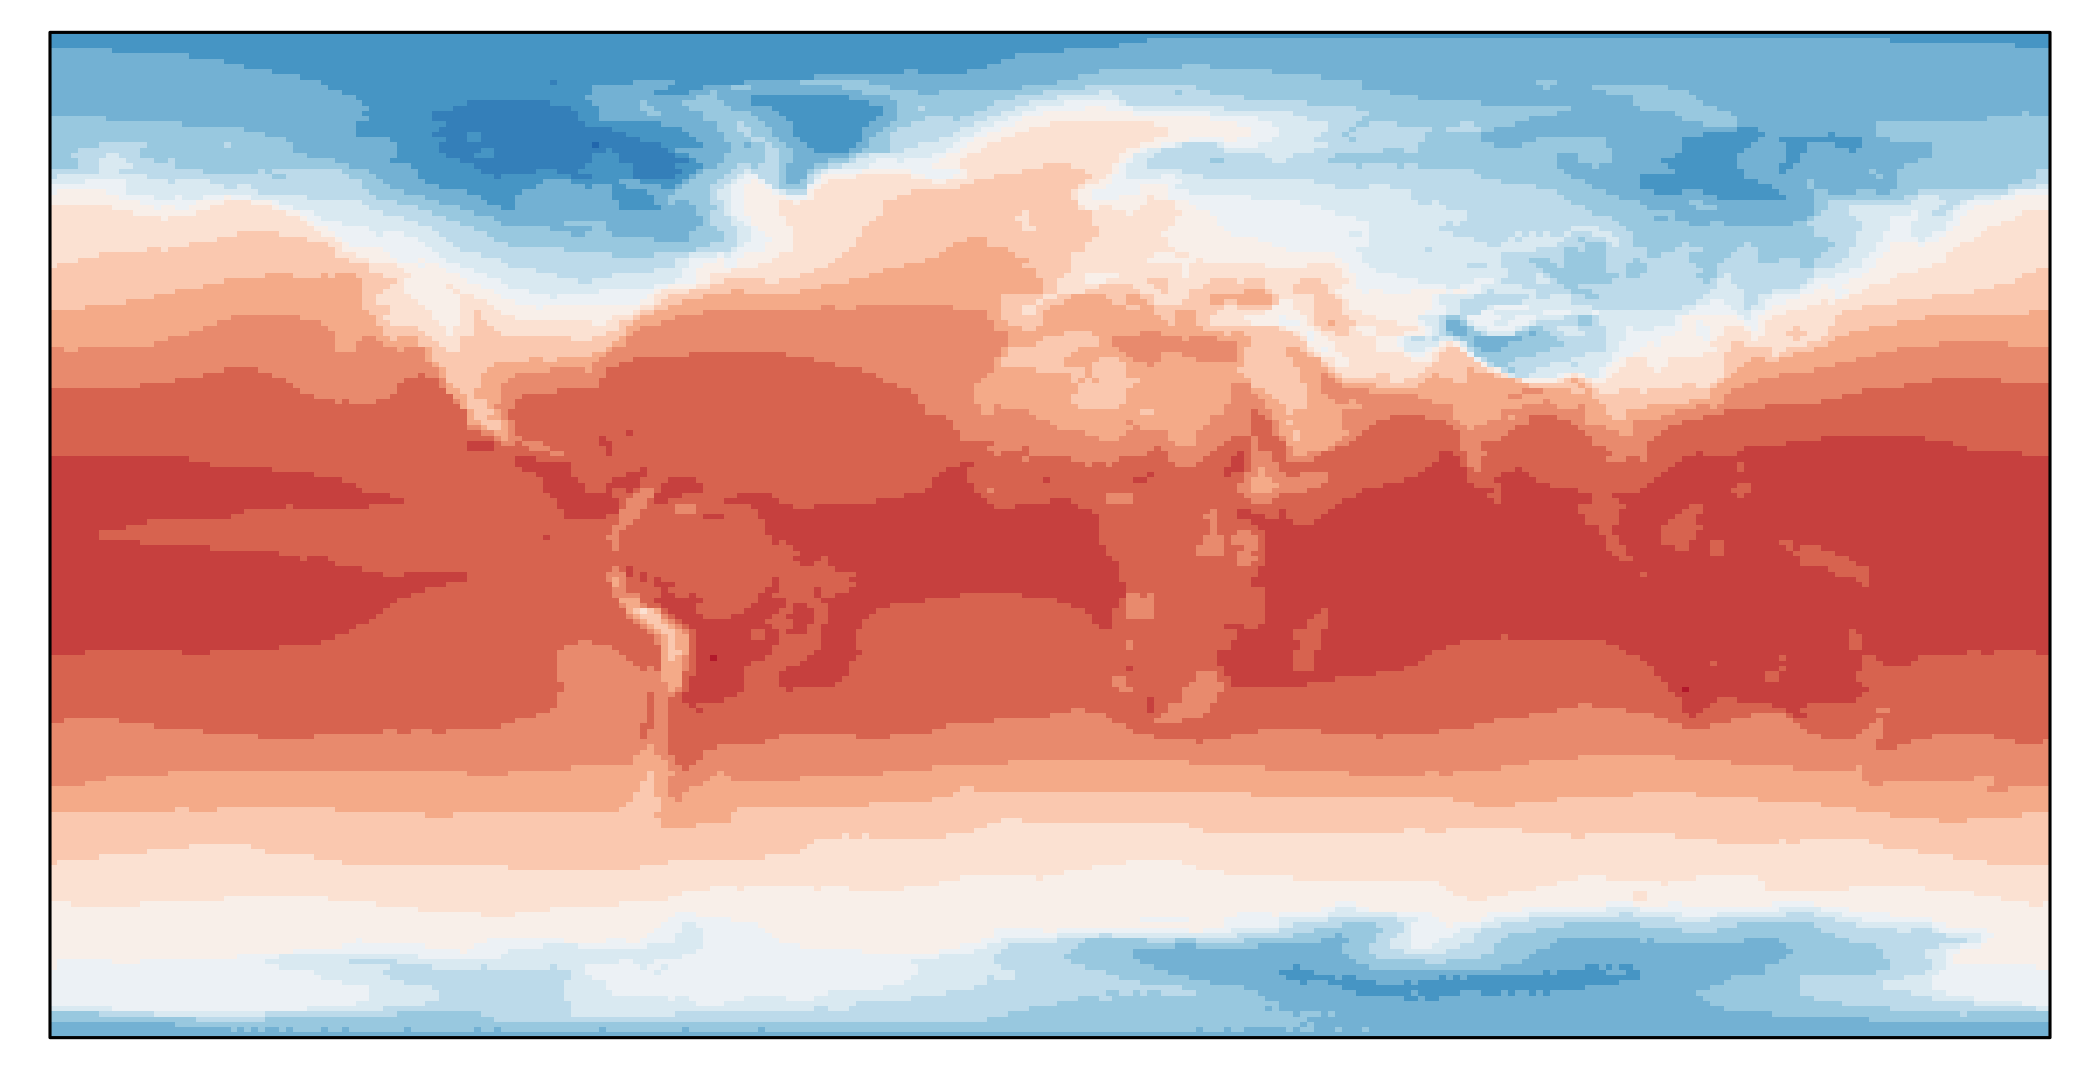
\includegraphics[width = .45\columnwidth]{images/ccsm4_temp}
    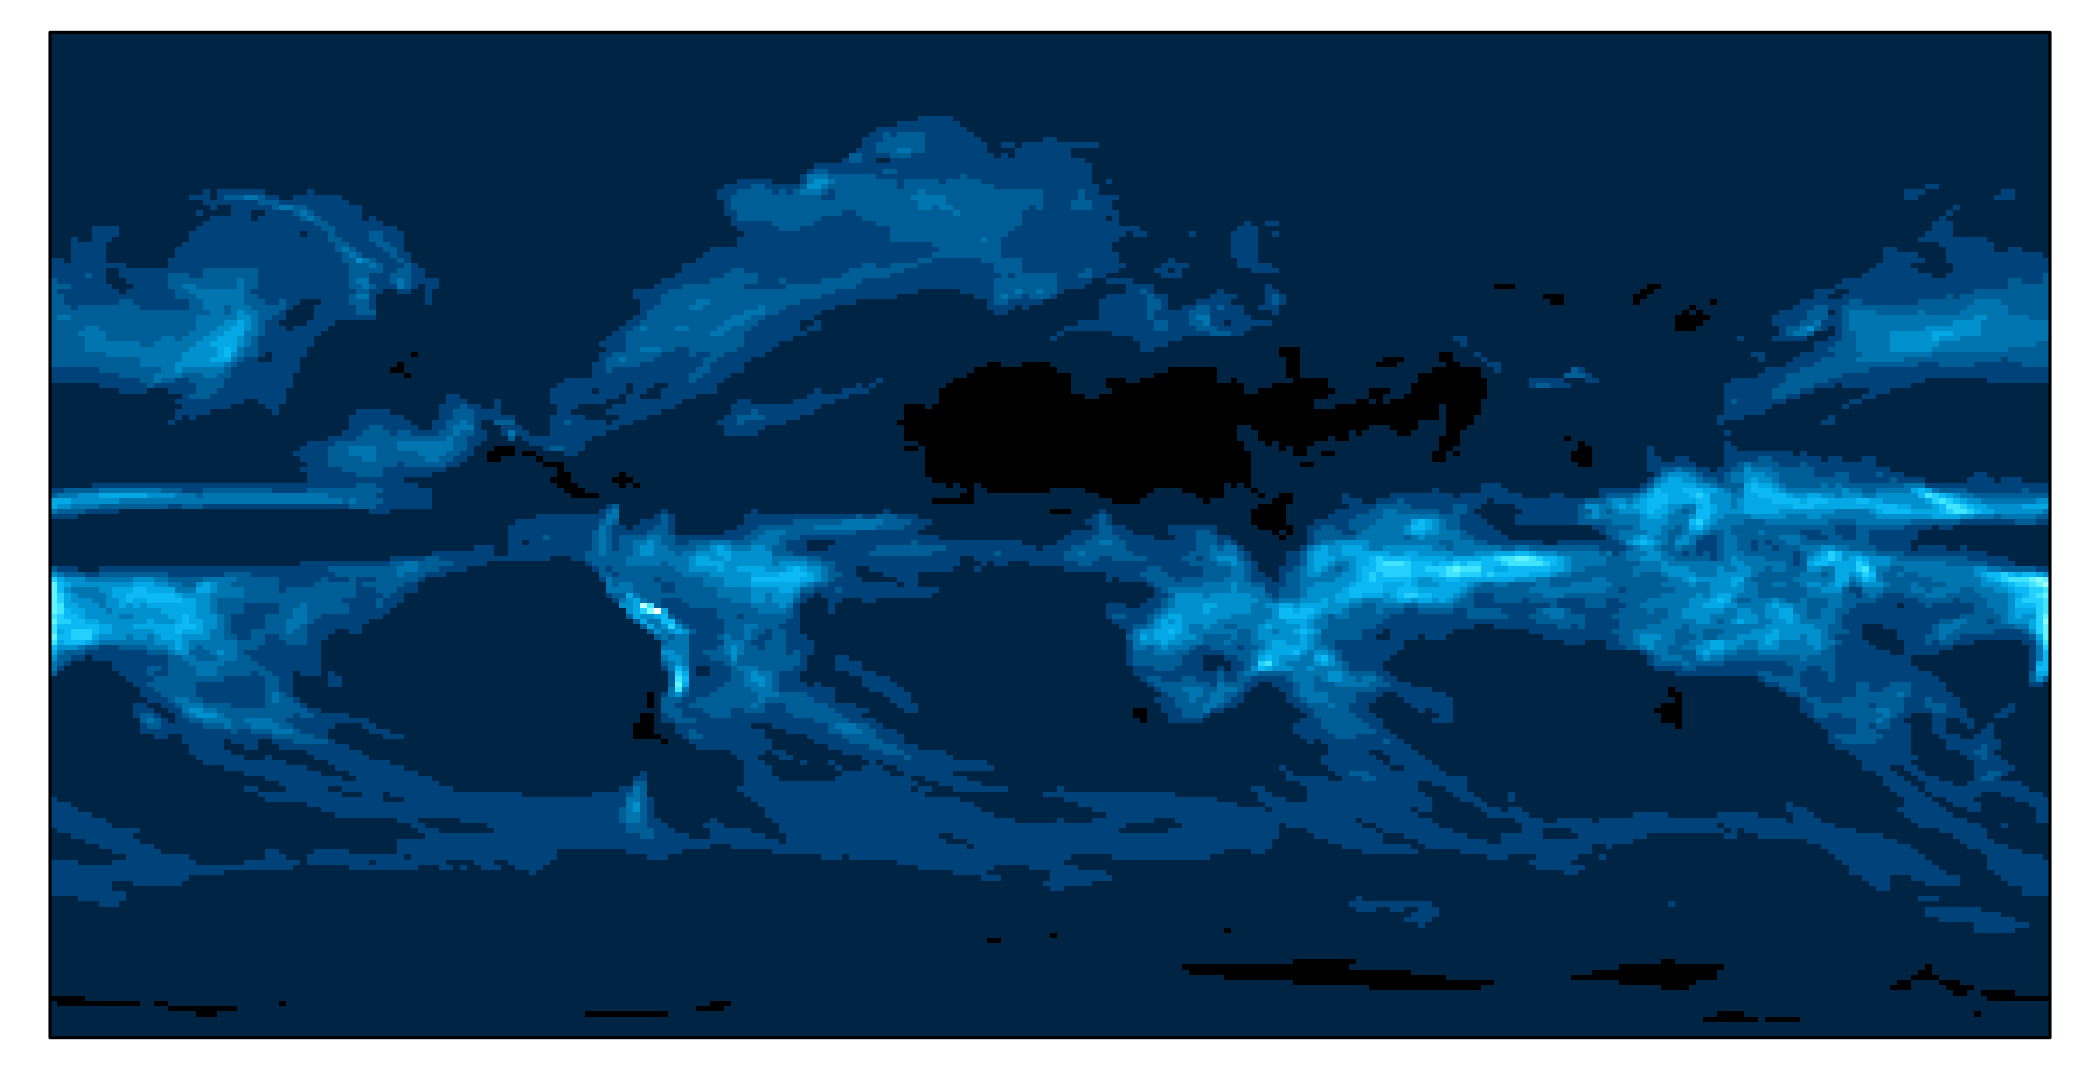
\includegraphics[width = .45\columnwidth]{images/ccsm4_prec}
    \captionof{figure}{Simulated global temperature (left) and precipitation (right) from CCSM4 LME.       }
%\end{center}
\medskip
\begin{multicols}{2}
\vspace*{\fill}
\noindent We use outputs from the Community Climate System Model 4, Last Millennium paleoclimate simulation \cite{Landrum2013LastCCSM4} to estimate temperature and precipitation for the AD 1200 -– 1400.\\
\\
\noindent We then calculate monthly water stress (precipitation -- potential evapotranspiration) over the U.S. Southwest from these simulation outputs, and compute a normalized annual drought index, the Standardized Precipitation Evapotranspiration Index (SPEI) \cite{Begueria2014StandardizedMonitoring}.
\vspace*{\fill}

\columnbreak
\begin{center}    
    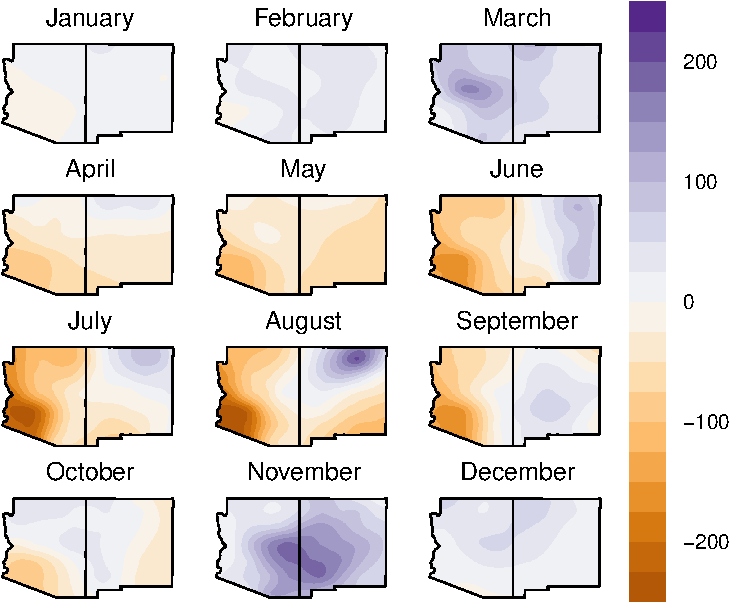
\includegraphics[width = .8\columnwidth]{images/water_stress}
    \captionof{figure}[skip=0pt]{One simulated year of water stress (mm).}
\end{center}
\end{multicols}

\medskip
\noindent Finally we decompose the space-time SPEI signal into \textit{empirical orthogonal functions} (EOFs)  \cite{Lorenz1956EmpiricalPrediction}. The drought EOFs represent pairs of regions that have maximally negatively correlated drought patterns. The leading six EOFs capture most of the variability in the simulated climate signal.\\
\begin{center}
    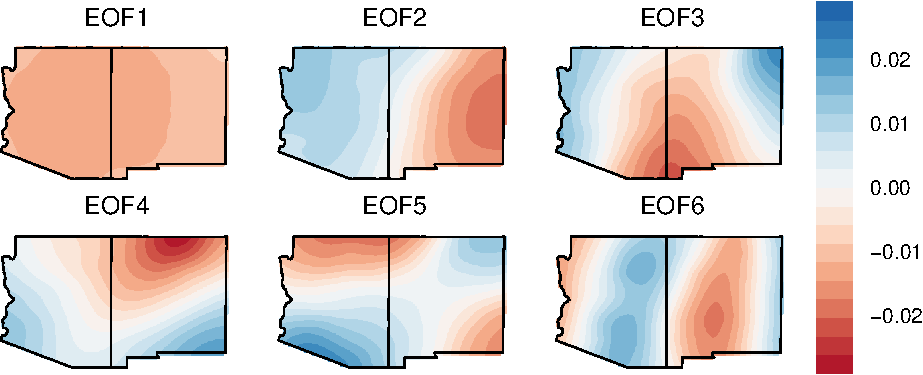
\includegraphics[width = .9\columnwidth]{images/eofs}
    \captionof{figure}{Leading six empirical orthogonal functions for the period AD 1200 -- 1400.}
\end{center}
\medskip


\columnbreak
\vspace*{\fill}
\subsection*{Social Network Proxies}
To estimate the topology of prehistoric social networks, we use data from the \textit{Southwest Social Networks} project. This dataset includes nearly 4.7 million ceramic artifacts and nearly 5,000 obsidian artifacts from nearly 1,000 well-dated sites in Arizona and western New Mexico for the period AD 1200 -- 1500 \cite{Mills2015a}. The similarity between artifact assemblages at each pair of sites is used as a proxy for the intensity of past social interaction.\\

\begin{center}
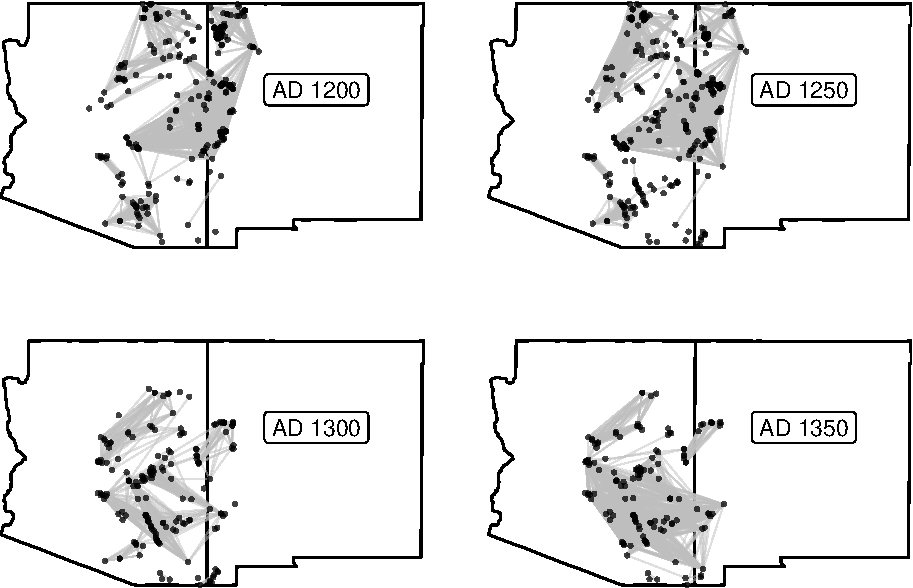
\includegraphics[width = .8\columnwidth]{images/swsn}
\captionof{figure}{Southwest Social Network data, only ties with similarity $>75\%$ shown.}
\end{center}
\vspace*{\fill}
\subsection*{Landscape Connectivity}
All else being equal, adjacent settlements will have stronger ties than more distant ones. To control for the effect of distance, we use a digital elevation model and Tobler's hiking function \cite{Tobler1993ThreeModeling} to calculate a least-cost network representing the shortest travel times between each pair of sites.\\
%\begin{multicols}{2}
%\noindent Tobler's hiking function \cite{Tobler1993ThreeModeling} models \textbf{walking speed} $W$ as a function of \textbf{slope} $S$:
%$$ W = 6 e^{-3.5|S + 0.05|} $$
%With this formula we calculate the shortest travel times between each site pair.
%\columnbreak
 
%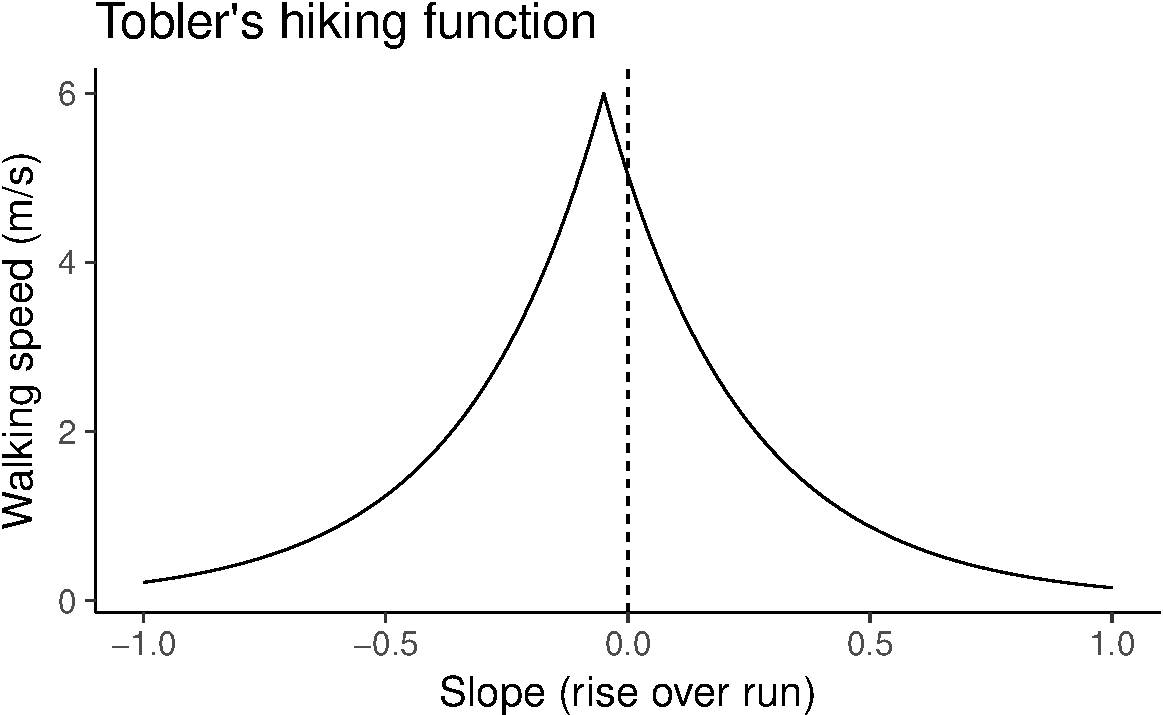
\includegraphics[width = .8\columnwidth]{images/tobler} 

%\end{multicols}


\begin{center}
    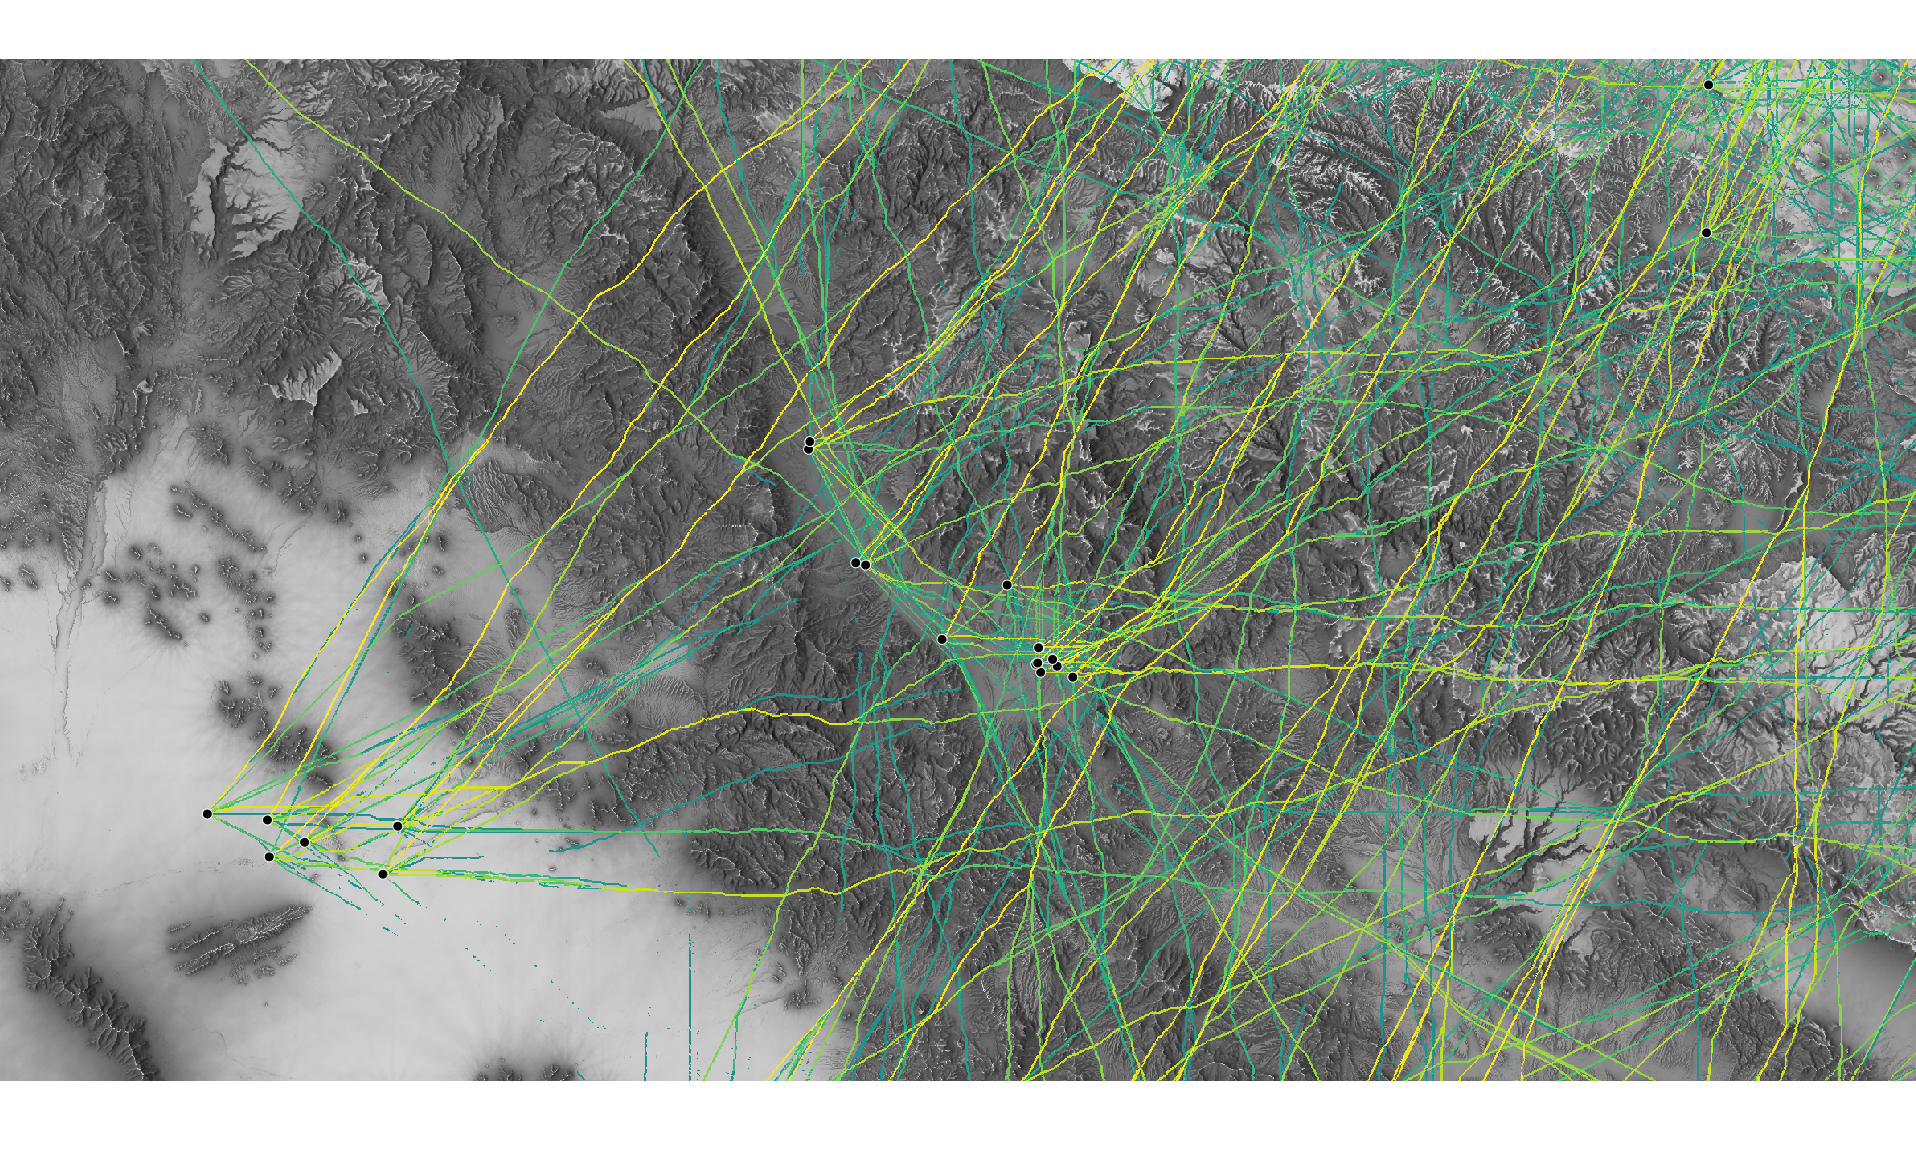
\includegraphics[width = .85\columnwidth]{images/fete}
        \captionof{figure}[skip=0pt]{Detail of least-cost network estimates.}

\end{center}
\vspace*{\fill}
\subsection*{Statistical Inference}
We fit a semiparametric, nonlinear regression (a \textit{generalized additive model}) to the data to assess the relationship between network dynamics and drought variability, while controlling for landscape connectivity and other environmental variables.
\vspace*{\fill}

\columnbreak

%%%Column 2




\columnbreak
\section*{Results}
\begin{multicols}{2}
\vspace*{\fill}
    The best fitting regression model includes travel time, water stress, elevation, and the 3rd and 4th EOFs as covariates. The strengths of network ties are significantly positively correlated with the third and fourth EOFs. While the remaining (non-significant) EOFs are stable through time, the spatial patterns of the third and fourth EOFs changed during the study period. Visual comparison between network dynamics and these EOFs suggests that \textbf{prehistoric social networks were sensitive to \textit{changes} in drought variability}.
\vspace*{\fill}

\columnbreak
    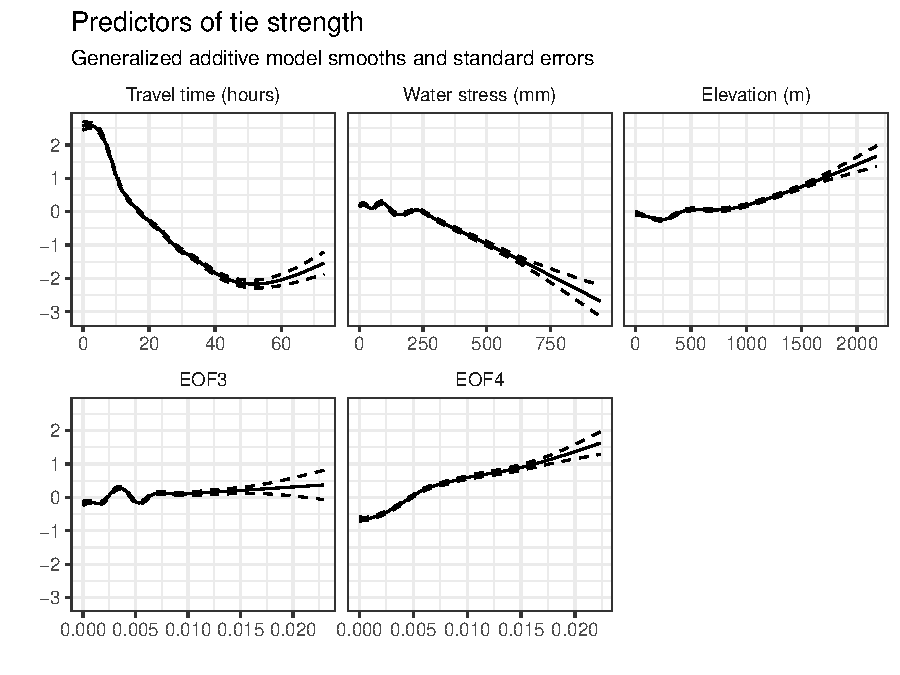
\includegraphics[width = \columnwidth]{images/smooths}

\end{multicols}

\vspace*{\fill}

\begin{center}
    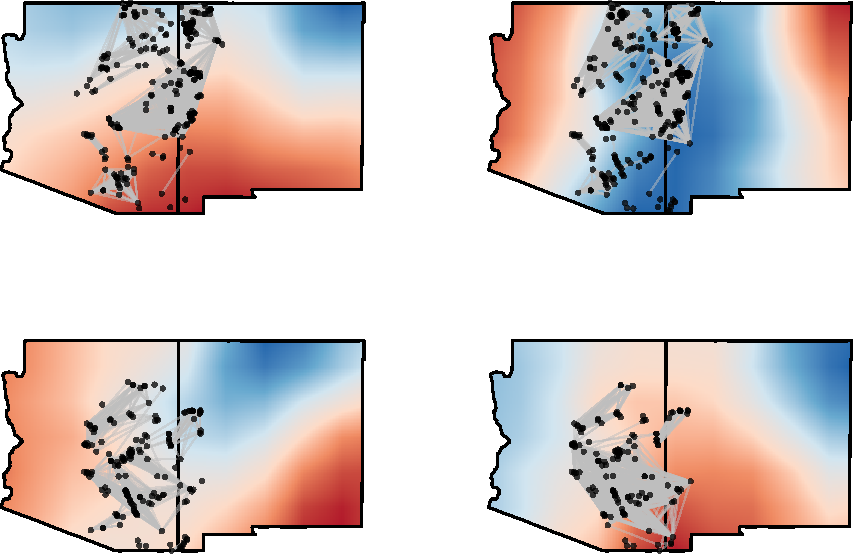
\includegraphics[width=.8\columnwidth]{images/eof3_net}
    %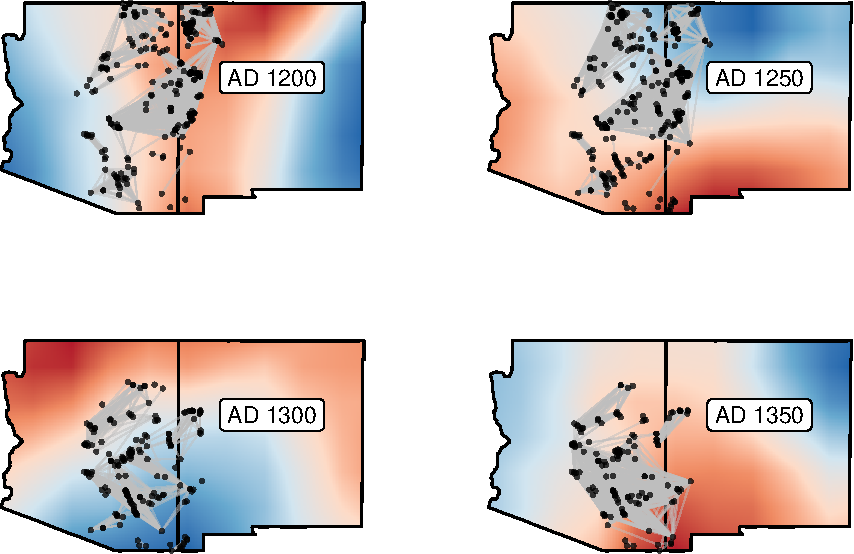
\includegraphics[width = .5\columnwidth]{images/eof4_net}
    \captionof{figure}{Relationship between network dynamics and changes in the 3rd EOF.}
    %\captionof{figure}{Relationship between network dynamics and changes in the fourth EOF.}
\end{center}

\vspace*{\fill}

Note that settlements are more likely to interact if they experience different patterns of climate \textit{variability}, not differences in \textit{average} climate. Water stress has a strong negative correlation with tie strength, and mean annual temperature and precipitation show no correlation at all. Counterintuitively, this suggests that the strong relationship between elevation difference and tie strength is not simply the result of climate contrasts, but rather more subtle ecophysiogrpahic variation. High-resolution statistically downscaled paleoclimate simulation data will help to further explore these patterns in future work.

\vspace*{\fill}

\footnotesize

\section*{Acknowledgements}
The Southwest Social Networks Project is funded through the Human and Social Dynamics Program of the National Science Foundation. The Community Climate System Model project is supported by the National Science Foundation and the Office of Science (Biological and Environmental Research program) of the U.S. Department of Energy.
We thank the developers of the following R packages central to this analysis: \texttt{raster, SPEI, spacetime, gdistance, igraph, mgcv}.

\bibliographystyle{abbrv}
\bibliography{mendeley.bib}

\end{multicols}

\end{document}
